% Adapted from the author's public Erdos Paper IV v1.23 series_template.tex.
% Layout provenance is recorded in 02_validation; the Markdown is semantic authority.
\documentclass[spanish,11pt,a4paper]{article}
\usepackage[margin=1in]{geometry}
\usepackage{fontspec}
\setmainfont{lmroman10-regular.otf}[BoldFont=lmroman10-bold.otf,ItalicFont=lmroman10-italic.otf,BoldItalicFont=lmroman10-bolditalic.otf]
\setsansfont{lmsans10-regular.otf}[BoldFont=lmsans10-bold.otf]
\setmonofont{lmmono10-regular.otf}[Scale=MatchLowercase]
\usepackage{amsmath,amssymb}
\providecommand{\mathscr}{\mathcal}
\usepackage[spanish,es-noshorthands,es-tabla]{babel}
\usepackage{microtype,parskip}
\usepackage{longtable,booktabs,array,calc}
\usepackage{xcolor,xurl}
\usepackage{hyperref,bookmark}
\usepackage{etoolbox,needspace}
\setcounter{secnumdepth}{-\maxdimen}
\setlength{\emergencystretch}{3em}
\providecommand{\tightlist}{\setlength{\itemsep}{0pt}\setlength{\parskip}{0pt}}
\newcounter{none}
\AtBeginEnvironment{longtable}{\Needspace{8\baselineskip}\small}
\pretocmd{\section}{\Needspace{5\baselineskip}}{}{}
\pretocmd{\subsection}{\Needspace{7\baselineskip}}{}{}
\pretocmd{\subsubsection}{\Needspace{6\baselineskip}}{}{}
\urlstyle{same}

\usepackage{graphicx}
\providecommand{\pandocbounded}[1]{#1}

\usepackage{float}

\clubpenalty=10000\widowpenalty=10000\displaywidowpenalty=10000
\usepackage{tikz}
\AtBeginEnvironment{longtable}{\Needspace{16\baselineskip}}
\hypersetup{pdftitle={Conteo de diseños de Steiner con perfiles de color prescritos},pdfauthor={Juan Pablo Traverso Gianini},pdflang={es},colorlinks=true,linkcolor=blue,urlcolor=blue,citecolor=blue}
\title{Conteo de diseños de Steiner con perfiles de color prescritos}
\author{Juan Pablo Traverso Gianini\\\small Investigador independiente, Santiago, Chile\\\small \href{mailto:jtraverso@gmail.com}{jtraverso@gmail.com}\\\small \href{https://orcid.org/0009-0003-6068-4096}{ORCID: 0009-0003-6068-4096}}\date{}\begin{document}\raggedbottom\maketitle
\begin{center}
\textbf{Paper III. Entropía combinatoria y conteo.}\\
\textbf{Preprint 1.0 --- 24 de noviembre de 2026.}\\
DOI: \url{https://doi.org/10.5281/zenodo.24501236}.\\
\href{https://github.com/jtraverso/latinon-entropy-ldp/tree/main/preprints/STEINER-PROFILES/05_formalization/lean}{Fuentes Lean en el repositorio de la serie}\end{center}
\subsection{Resumen}\label{resumen}

Dada una partición de \(n\) puntos etiquetados en \(k\) clases de color de tamaño lineal, contamos los diseños de Steiner \(S(2,q,n)\) que tienen exactamente \(m_\tau\) bloques de cada multiconjunto de colores \(\tau\). Para \(q\ge3\) y \(k\) fijos, la estimación es uniforme sobre las cuotas enteras que satisfacen los márgenes de pares y la divisibilidad ordinaria, siempre que cada tipo represente una fracción positiva fija de los bloques. El coste de prescribir las cuotas es, en escala logarítmica, el número de bloques multiplicado por la entropía relativa del perfil respecto de la ley de un bloque uniforme. Damos errores con ahorro de potencia en ambas direcciones. La construcción inferior reserva pequeños grafos con dos descomposiciones posibles, que permiten ajustar el histograma entero después de completar el diseño. Deducimos un principio de grandes desviaciones para el histograma de un diseño etiquetado uniforme, sobre el politopo de márgenes. En un perfil de frontera, la aproximación por perfiles interiores da la cota inferior para cada entorno abierto.

MSC 2020: 05B05, 05A16, 60F10. Palabras clave: diseños de Steiner; perfiles de color; enumeración; entropía relativa; grandes desviaciones.

\begin{center}\rule{0.5\linewidth}{0.5pt}\end{center}

\subsection{1. Introducción}\label{introducciuxf3n}

\subsubsection{1.1 Antecedentes}\label{antecedentes}

En un sistema de Steiner \(S(2,q,n)\) cada par de puntos pertenece a un único bloque de tamaño \(q\). Si los puntos se han coloreado de rojo y azul, un bloque con \(j\) puntos rojos consume \(\binom j2\) pares rojos y \(j(q-j)\) pares mixtos. Aumentar el número de bloques de ese tipo obliga, por tanto, a modificar otras cuotas. Incluso después de cuadrar las cuentas de pares, queda por decidir si los bloques pueden colocarse sobre los puntos dados y cuánto cuesta imponer esa distribución.

El Paper I de la serie cuenta cuadrados latinos en un entorno de un Latinon prescrito {[}6{]}. El Corolario 1.6 del Paper II da las grandes desviaciones del perfil de un sistema triple {[}2{]}. Keevash {[}1{]} contó los diseños sin prescribir las cuotas. Para \(q=3\), el Teorema 1.5 del Paper II {[}2{]} identifica la penalización entrópica de un histograma prescrito. Aquí tratamos todo \(q\ge3\) fijo. La misma matriz que impone las condiciones necesarias de pares determina los intercambios que utilizaremos para obtener el histograma exacto.

\subsubsection{1.2 El teorema de conteo}\label{el-teorema-de-conteo}

Fijemos una paleta de \(k\) colores y una coloración de los puntos etiquetados de \([n]\), con \(n_i\) puntos de color \(i\). Un tipo \(\tau\) se especifica mediante sus multiplicidades \(\tau_i\ge0\), que suman \(q\). Escribimos \(r=\binom q2\). El número de bloques de un diseño y el número de bloques \emph{posibles} de tipo \(\tau\) son, respectivamente, \[b=\frac{\binom n2}{r},\qquad N_\tau=\prod_i\binom{n_i}{\tau_i}.\] Para cada multiconjunto \(u\) de dos colores, sea \(A_{u,\tau}=\prod_i\binom{\tau_i}{u_i}\). Si \(m_\tau\) es la cuota del tipo \(\tau\), la ecuación de márgenes es \((Am)_u=\prod_i\binom{n_i}{u_i}\) para todo \(u\). Al sumar sobre \(u\) se obtiene \(\sum_\tau m_\tau=b\). Denotemos por \(N(m)=N_\chi(m)\) el número de diseños con ese histograma, manteniendo fija la coloración.

Hay dos distribuciones naturales sobre los tipos. Un bloque elegido en el diseño tiene ley \(Q_\tau=m_\tau/b\). Un \(q\)-subconjunto elegido entre todos los posibles tiene ley \(P_\tau=N_\tau/\binom nq\). Escribimos \(D(Q\|P)=\sum_\tau Q_\tau\log(Q_\tau/P_\tau)\) con la contribución cero cuando \(Q_\tau=0\). Cada arista pertenece a \(d_0=\binom{n-2}{q-2}\) bloques posibles. Definimos \[\Phi(m)=b\,[\log d_0-(r-1)-D(Q\|P)]. \tag{1}\]

\textbf{Teorema 1.1.} Fijados \(q\ge3\), \(k\), \(\rho>0\) y \(\kappa>0\), existen \(C\) y \(n_0\) tales que lo siguiente vale para \(n\ge n_0\). Supongamos que \(r\mid\binom n2\), que \(q-1\mid n-1\) y que \(n_i\ge\rho n\) para cada color. Para toda cuota entera \(m\) con los márgenes indicados y \(m_\tau\ge\kappa b\) para cada tipo, existe un diseño y \[\Phi(m)-C n^{2-z}\log n\ \le\ \log N(m)\
 \le\ \Phi(m)+C n^{2-1/(r-1)},\qquad
 z=\frac{1}{(4r-1)(2q-1)+2}. \tag{2}\] La cota \(N(m)\le\exp(\Phi(m)+C n^{2-1/(r-1)})\) se extiende a todas las cuotas enteras no negativas con esos márgenes.

Los cerrados de la sección 10 pueden incluir perfiles con tipos de masa cero; allí usaremos la cota superior. Para tamaños de bloque \(3,4,5\), el exponente inferior \(z\) vale \(1/57,1/163,1/353\), respectivamente. Estos ahorros son asintóticos para \(q\) fijo.

\subsubsection{1.3 Trabajos previos y estrategia de demostración}\label{trabajos-previos-y-estrategia-de-demostraciuxf3n}

Con un solo color recuperamos el término principal del Teorema 6.1 de Keevash {[}1{]}. Sus trabajos sobre diseños coloreados y dirigidos dan un marco de existencia para descomposiciones con colores de aristas y estructuras partitas {[}7, 8{]}. Kwan, Sah y Sawhney dan cotas superiores para el número de descomposiciones con números prescritos de cliques de cada tamaño {[}9, §2.2{]}. Aquí el tamaño es fijo y el histograma distingue los colores de los vértices. Sobre el proceso voraz de matching véanse {[}1, 10{]}.

Para la cota inferior, asignamos a cada bloque posible de tipo \(\tau\) el peso \(m_\tau/N_\tau\). La suma de los pesos de los bloques que contienen una arista vale uno. En una elección sucesiva de bloques, estos pesos favorecen los tipos que queremos obtener. Sin embargo, cuando la última arista queda cubierta ya no hay libertad para elegir otro bloque. Por eso separamos de antemano un pequeño grafo con varias descomposiciones. El Lema 3.1 explica por qué basta esta reserva. Las diferencias de histogramas de sus intercambios generan todos los cambios enteros permitidos por los márgenes de pares. La prueba inferior consta de tres operaciones que requieren controles distintos: preparar los pesos y los intercambios, seguir las frecuencias durante la elección aleatoria y contar cuántas elecciones dan el mismo diseño.

{\def\LTcaptype{none} % do not increment counter
\begin{longtable}[]{@{}
  >{\raggedright\arraybackslash}p{(\linewidth - 4\tabcolsep) * \real{0.3333}}
  >{\raggedright\arraybackslash}p{(\linewidth - 4\tabcolsep) * \real{0.3333}}
  >{\raggedright\arraybackslash}p{(\linewidth - 4\tabcolsep) * \real{0.3333}}@{}}
\toprule\noalign{}
\begin{minipage}[b]{\linewidth}\raggedright
Aristas apartadas
\end{minipage} & \begin{minipage}[b]{\linewidth}\raggedright
Elección al completar
\end{minipage} & \begin{minipage}[b]{\linewidth}\raggedright
Cantidad controlada
\end{minipage} \\
\midrule\noalign{}
\endhead
\bottomrule\noalign{}
\endlastfoot
Reserva & Extender las aristas descubiertas a cliques & Grado máximo del resto \\
Omniabsorbedor & Descomponerlo junto al resto divisible de la reserva & Cobertura de todos los pares \\
Celdas de intercambio & Alternar dos descomposiciones de las mismas aristas & Histograma entero exacto \\
\end{longtable}
}

Tabla 1. Función de los tres conjuntos de aristas reservados antes del empaquetamiento aleatorio voraz.

\subsection{2. Cómo reparar los pesos al retirar aristas}\label{cuxf3mo-reparar-los-pesos-al-retirar-aristas}

Sea \(\lambda_B=m_\tau/N_\tau\) para un bloque \(B\) de tipo \(\tau\). La suma de las cargas de todas las aristas del tipo \(u\) es \((Am)_u\). Dentro de ese tipo, cualquier arista puede llevarse a cualquier otra permutando puntos del mismo color. Todas tienen, pues, carga uno. Además \(\lambda_B\) está entre dos múltiplos positivos de \(n^{2-q}\), uniformemente en \(B\).

Las aristas reservadas eliminan bloques enteros del proceso. Para restaurar las cargas en el grafo restante \(J\) usamos su matriz de incidencia \(H_J\), con filas indexadas por aristas y columnas por copias de \(K_q\) contenidas en \(J\). Si \(S_J=d_0^{-1}H_JH_J^\top\) es invertible, entonces \(R_J=d_0^{-1}H_J^\top S_J^{-1}\) es una inversa derecha de \(H_J\). Lo importante es cuánto peso puede concentrar esa reparación en un solo bloque.

\textbf{Lema 2.1 (Corrección de las cargas).} Para cada \(q\ge3\) fijo existen \(\varepsilon_q>0\) y \(n_q\) tales que, si \(n\ge n_q\) y el grafo retirado tiene grado máximo a lo sumo \(\varepsilon_q n\), la matriz de incidencia de los cliques restantes tiene una inversa derecha que satisface ambas cotas de (3).

\textbf{Demostración.} En el grafo completo, las permutaciones de los puntos tienen tres órbitas sobre los pares ordenados de aristas. Sus matrices invariantes son constantes en esas tres clases. Las matrices \(I,K,E\) que se introducen a continuación distinguen las clases y generan su álgebra, el álgebra de Johnson sobre los pares.

Una entrada de \(S_0\) depende únicamente de si las dos aristas coinciden, se cortan o son disjuntas. En ese orden, los tres valores son \(1\), \((q-2)/(n-2)\) y \((q-2)(q-3)/((n-2)(n-3))\). Se obtienen completando la unión de los extremos a un \(q\)-conjunto. La inversa \(U\) tiene las mismas tres clases de entradas. Con \(D_0=q(q-1)(n-q)(n-q-1)\), sus valores son \[\begin{gathered}u_0=\frac{q(q-1)n^2-q(7q-9)n+4(3q^2-5q+1)}{D_0},\\[3pt]
 u_1=-\frac{(q-2)(qn-4q+2)}{D_0},\quad
 u_2=\frac{2(q-2)}{q(n-q)(n-q-1)} .\end{gathered}\] En efecto, si \(T\) es la incidencia arista--vértice, el producto \(K=TT^\top\) tiene diagonal dos y entrada uno en las aristas adyacentes. Con \(E\) la matriz de unos se tiene \(K^2=(n-2)K+4E\), \(KE=2(n-1)E\) y \(E^2=\binom n2E\). Escribir \(S_0\) y \(U\) en la base \(I,K,E\) y multiplicar da \(S_0U=I\). Una columna de \(U\) contiene una entrada \(u_0\), \(2(n-2)\) entradas \(u_1\) y \(\binom{n-2}2\) entradas \(u_2\). Para \(n\ge2q^2\) su suma absoluta es a lo sumo cuatro (se comprueba sustituyendo las tres entradas anteriores). En el límite esa suma tiende a \(1+2(q-2)/(q-1)+(q-2)/q<4\).

Supongamos que las aristas retiradas forman un grafo \(F\) de grado máximo \(t\). En cada columna de \(S_0[F,J]\), las aristas adyacentes contribuyen \(O(t/n)\) y las disjuntas \(O(nt/n^2)\). Si \(\beta\) es la mayor suma de columna de ese bloque, entonces \(\|S_0[J,J]-S_J\|_1\le r\beta\): cada clique perdido contiene una arista de \(F\) y aporta a lo sumo \(r\) incidencias. Al restringir la identidad del completo resulta \(\|U[J,J]S_J-I\|_1\le4(r+1)\beta\). En cada columna contribuyen a lo sumo \(2t\) aristas retiradas adyacentes y \(nt/2\) disjuntas. Para \(C_q=2(q-2)(q-1)\), las cotas anteriores dan \(\beta\le C_q t/n\) para \(n\ge2q^2\). Tomando \(n_q=2q^2\) y \(\varepsilon_q=1/(8(r+1)C_q)\), el error es a lo sumo \(1/2\). La serie geométrica da \(\|S_J^{-1}\|_1\le8\) y, por simetría, la misma cota en norma infinito. En particular, \[\|R_J h\|_1\le8\|h\|_1,\qquad
 \|R_J h\|_\infty\le 8r\,d_0^{-1}\|h\|_\infty . \quad\square\tag{3}\]

También podemos reparar el histograma. Para una dirección \(g\in\ker A\), el peso \(g_\tau/N_\tau\) sobre los bloques de tipo \(\tau\) tiene cargas cero e histograma \(g\). Para cada vector de una base fija del núcleo, restringimos estos pesos a \(J\) y anulamos las cargas residuales mediante (3). Sus histogramas difieren de los vectores de la base en \(O(t/n)\) y sus pesos individuales son \(O(n^{-q})\). En coordenadas de la base, la matriz de histogramas es una perturbación de la identidad de dimensión fija. Invertirla permite imponer un cambio de tamaño \(O(nt)\) con pesos adicionales \(O(nt\,n^{-q})\). Esto representa una fracción \(O(t/n)\) de la semilla inicial y conserva su positividad.

\subsection{3. Intercambios que generan las correcciones enteras}\label{intercambios-que-generan-las-correcciones-enteras}

\textbf{Lema 3.1 (Generación entera por intercambios).} Para \(q,k\) fijos existe una familia finita de intercambios entre descomposiciones de las mismas aristas cuyas diferencias de histogramas generan \(\ker A\) sobre los enteros. Un defecto \(h\) en el núcleo entero se corrige con a lo sumo \(C_{q,k}\|h\|_1\) intercambios, admitiendo ambas orientaciones.

\textbf{Demostración.} Fijemos un color de referencia, el \(0\). Tomemos un primo \(\ell\ge q\) y pendientes distintas \(s_1,\ldots,s_q\) en \(\mathbb F_\ell\). Sobre los grupos \(\{i\}\times\mathbb F_\ell\) consideremos los bloques \[B_{x,y}=\{(i,x+s_i y):1\le i\le q\},\qquad (x,y)\in\mathbb F_\ell^2 .\] Dos puntos de grupos distintos determinan \(x,y\) mediante dos ecuaciones de pendientes diferentes. Por ello estos bloques descomponen el grafo completo \(q\)-partito. Una permutación dentro de un grupo produce una segunda descomposición de sus mismas aristas.

Para un tipo \(\tau\) con \(d\ge3\) puntos de color distinto de \(0\), asignemos esos colores a los puntos de coordenada cero de \(d\) grupos y pintemos el resto con el color de referencia. Sólo \(B_{0,0}\) contiene los \(d\) puntos señalados. Intercambiemos ahora las coordenadas cero y uno en uno de esos grupos, trasladando los bloques y dejando fijos los colores. Dos de los puntos señalados siguen forzando \(x=y=0\), pero el bloque correspondiente ha perdido el tercero. La diferencia \(g_\tau\) de los histogramas tiene coordenada uno en \(\tau\). Las demás coordenadas que cambian tienen menos de \(d\) puntos señalados. Además \(Ag_\tau=0\), pues se cubren las mismas aristas.

Dado un defecto entero en \(\ker A\), eliminamos sus coordenadas en orden decreciente de \(d\). El coeficiente principal uno permite hacerlo con múltiplos enteros de los \(g_\tau\). Entre los tipos restantes, el margen de cada par de colores no nulos \(i,j\) determina la coordenada \(0^{q-2}ij\), incluso cuando \(i=j\). Una vez anuladas esas coordenadas, los márgenes \(0i\) y finalmente \(00\) anulan las demás. Por tanto los \(g_\tau\) forman una base entera y, por dimensión fija, la suma absoluta de los coeficientes necesarios es a lo sumo \(C_{q,k}\) veces la norma uno del defecto. \(\square\)

Por ejemplo, tomemos \(q=4\) y las pendientes \(0,1,2,3\) en \(\mathbb F_5\). En cada uno de los tres primeros grupos coloreamos de rojo el punto de coordenada cero y dejamos azules todos los demás. Los 25 bloques tienen histograma \((12,12,0,1,0)\) en orden creciente de número de puntos rojos. Al intercambiar las coordenadas cero y uno del primer grupo obtenemos \((13,9,3,0,0)\) sobre los mismos pares. Desaparece el único bloque con tres puntos rojos y aparecen tres con dos.

Reservamos \(O(Bn^{2-z})\) copias de estas celdas, con ambas orientaciones. Se colocan con aristas disjuntas y grado máximo \(D_Bn^{1-z}\). En efecto, los vértices próximos a ese límite son \(O(Bn/D_B)\) por suma de grados. Elegimos \(D_B\) de modo que ocupen menos de un cuarto de la clase más pequeña. Cada punto de una nueva celda debe evitar además los vecinos prohibidos de un número acotado de puntos ya elegidos. Son \(o(n)\) exclusiones adicionales. Siempre queda un punto del color solicitado.

\subsection{4. La energía del proceso aleatorio}\label{la-energuxeda-del-proceso-aleatorio}

En el grafo \(J\) provisto de pesos reparados \(\mu_B\), elegimos sucesivamente un bloque libre con probabilidad proporcional a su peso y retiramos sus \(r\) aristas. Tras \(i\) elecciones quedan \(rm_i\) aristas, donde \(m_i=b_J-i\) y \(b_J=|E(J)|/r\). Escribimos \(p_i=m_i/b_J\) y \(k_i=p_i^{r-1}\). Para una arista libre, \(k_i\) es la carga prevista: fijada esa arista, el bloque sólo sobrevive si siguen libres las otras \(r-1\).

Sean \(a_e\) el indicador de arista libre, \(d_e\) su carga disponible y \(Z\) el peso total disponible. Medimos las desviaciones por \(x_e=d_e-k_i a_e\) y \(X=\sum_e x_e^2\). Como cada bloque contribuye a \(r\) cargas, \[s:=\sum_e x_e=r(Z-m_i k_i),\qquad |s|\le\sqrt{rm_i X}.\] Basta, pues, controlar una suma de cuadrados para estimar el denominador de cada probabilidad de elección.

La estimación de deriva utiliza una desigualdad que conserva el signo del término de interacción. En un bloque disponible, con cargas positivas \(d_1,\ldots,d_r\) y \(x_j=d_j-k\), se tiene \[\sum_j x_j^2-2\Big(\sum_j x_j\Big)^2
       \le (2r-1)k\sum_j x_j^2/d_j . \tag{4}\] Por homogeneidad tomemos \(k=1\) y pongamos \(S=\sum d_j\), \(T=\sum 1/d_j\). Si \(S\le2r-1\), basta usar \(d_j\le S\) en cada sumando. Para \(S\ge2r-1\) usamos \((S^2-\sum d_j^2)T\ge r(r-1)S\). Al expandir, los índices repetidos contribuyen \(2(r-1)S\) y cada terna distinta aporta \(2(ab/c+ac/b+bc/a)\ge2(a+b+c)\). Esta última desigualdad se obtiene sumando los cuadrados de las diferencias entre \(ab,ac,bc\). Sustituida la cota de \(\sum d_j^2\), basta probar \[(2r-1)T^2+[S^2-(2r-1)S-r(2r-1)]T+r(r-1)S\ge0.\] Al multiplicar por \(S^2\) y poner \(V=ST-r^2\), \(U=S-(2r-1)\), la expresión es \((2r-1)V^2+[U^3+(4r-2)U^2+(2r-1)(r-1)U+r(2r-1)]V+r(S-r)^2(2r-1)(S+r)\). Ambos parámetros son no negativos, el primero por Cauchy. Esto prueba (4).

Sea \(S_{ef}\) el peso de los bloques disponibles que contienen \(e\) y \(f\). Sumando (4) sobre los bloques con peso \(\mu_B\), obtenemos \(\sum_e d_ex_e^2-2x^\top Sx\le(2r-1)kX\): en la suma de la derecha los pesos de los bloques que contienen \(e\) cancelan el denominador \(d_e\). Esta unidad de holgura en el coeficiente permite absorber los errores al pasar al instante siguiente.

Más precisamente, para \(m=m_i\), \(k=k_i\) y \(\eta=k_i-k_{i+1}\), el descenso principal de las cargas aporta \((\sum d_ex_e^2-2x^\top Sx)/Z\). Al expandir el cuadrado de la nueva desviación hay que contar una sola vez cada bloque perdido. El peso común de dos aristas distintas está acotado por \(\beta=O(1/n)\), pues juntas fijan al menos tres vértices. El error de primer orden en una carga está acotado, antes de dividir por \(Z\), por \(\gamma d_e\) con \(\gamma=r^2\beta\). Fuera del bloque elegido, cada pérdida \(H_e\) es a lo sumo \(r\beta\) y \(\sum_e H_e\le r^2\), de modo que \(\sum_e H_e^2=O(1/n)\).

Mientras \(X/(rmk^2)=O(n^{-2z})\), tenemos \(Z=mk(1+O(n^{-z}))\). Si \(C\) es el bloque elegido, escribamos \(\rho_e\) para la corrección por intersecciones múltiples, definida por \(\sum_C\mu_C H_e(C)=(Sd)_e-\rho_e\) sobre los bloques disponibles. Tenemos \(0\le\rho_e\le\gamma d_e\). Sean \(H\) y \(W\) las sumas de \(H_e(C)\) y \(H_e(C)^2\), respectivamente, sobre las aristas libres fuera de \(C\). Para esas aristas la nueva desviación es \(x_e-H_e(C)+\eta\); para las de \(C\) es cero. Al elevar al cuadrado, restar \(X\) y promediar se obtiene \[\begin{aligned}
 \mathbb E[\Delta X\mid\mathcal F_i]
 &=\frac{\sum_e d_e x_e^2-2x^\top Sx-2(r-1)k(X+ks)+2x^\top\rho}{Z}\\
 &\quad+2\eta\,[s-(X+ks)/Z]+\mathbb E[W-2\eta H\mid\mathcal F_i]
             +r\eta^2(m-1). 
\end{aligned}\tag{5}\] El último sumando cuenta las \(r(m-1)\) aristas que siguen libres. El error lineal de intersecciones queda acotado por \(2\gamma(X+k\sqrt{rmX})/Z\). La última expresión es \(o(1)X/m+\varepsilon X/m+O_\varepsilon(\gamma^2)\), ya que \(\gamma/k=o(1)\). El cambio del valor de referencia satisface \(0\le(r-1)k/m-\eta=O_r(k/m^2)\). En la expansión, los términos en \(s\) se agrupan como \[2s[\eta-(r-1)k/m]+\frac{2(r-1)k}{Z}\,[s^2/(rm)-X].\] El segundo es no positivo por Cauchy. El primero y el término cuadrático en \(\eta\) cuestan a lo sumo \(\varepsilon X/m+O_\varepsilon(1/m)\). Hasta el horizonte utilizado abajo, \(1/m=O(1/n)\). Tomando \(\varepsilon\) suficientemente pequeño en función de \(r\), la holgura de (4) da \[\mathbb E[X_{i+1}-X_i\mid\mathcal F_i]\le (2r/m_i)X_i+C/n . \tag{6}\]

\subsection{5. Cuántos bloques de cada tipo se han elegido}\label{cuuxe1ntos-bloques-de-cada-tipo-se-han-elegido}

Dos escalas intervienen en la parada. El exponente \(a\) fija la fracción de aristas que se deja a la reserva y \(z\) fija la precisión relativa que requieren las frecuencias de tipos. Al bajar \(p_i\), disminuye la carga de referencia \(p_i^{r-1}\) y un mismo error absoluto tiene mayor efecto. Elegimos el horizonte para que el error relativo de energía todavía controle las probabilidades de elección.

Detenemos las elecciones en \(T=\lfloor b_J(1-n^{-a})\rfloor\), con \(a=(2q-1)z\). Para controlar todo el intervalo multiplicamos la energía por \(p_i^{2r}\). El factor compensa el crecimiento permitido en (6), pues \((1-1/m)^{2r}(1+2r/m)\le1\) para \(m\ge1\). Congelamos \(Y_i=p_i^{2r}X_i\) al cruzar por primera vez \(An\), conservando el valor que alcanzó al cruzarlo. Como \(X_0=0\), sumar las derivas da \(\mathbb E Y_T\le CT/n=O(n)\). La probabilidad de cruzar el umbral es a lo sumo \(O(1/A)\).

Antes de cruzarlo, \(X_i\le Anp_i^{-2r}\) y por tanto \(X_i/(rm_i k_i^2)=O(An^{-1}p_i^{-(4r-1)})\). La identidad \((4r-1)a+2z=1\) convierte esta cota en \(O(An^{-2z})\) hasta \(T\). Así se justifica la hipótesis empleada para la deriva en cada paso activo, incluido el paso que puede provocar la parada.

Sea \(R_\tau=Z_\tau/Z\) la fracción de peso disponible del tipo \(\tau\). Si una elección retira masa total \(U\) y masa \(V\) del tipo \(\tau\), la nueva fracción es \((Z_\tau-V)/(Z-U)\). Por tanto su incremento es \((R_\tau U-V)/(Z-U)\). Cada arista del bloque elegido tenía carga a lo sumo uno, de modo que \(0\le V\le U\le r\). Mientras \(Z\ge2r\), sustituir \(Z-U\) por \(Z\) en el denominador del incremento cuesta a lo sumo \(2r^2/Z^2\).

¿Por qué es pequeña la esperanza de \(R_\tau U-V\)? Sea \(d_{e,\tau}\) la carga en \(e\) debida al tipo \(\tau\). Contar la masa retirada por cada arista compartida da \(\sum_e d_e^2/Z\) para \(U\) y \(\sum_e d_e d_{e,\tau}/Z\) para \(V\), con un exceso cuando dos bloques comparten varias aristas. La contribución de ese exceso a la deriva del cociente está acotada por \(\gamma/Z\). En el término restante se puede centrar \(d_e\) en \(k_i\), pues \(\sum_e(d_{e,\tau}-R_\tau d_e)=rZ_\tau-R_\tau rZ=0\). Así, el numerador centrado queda acotado en valor absoluto por \[\sum_e d_e|d_e-k_i|\le X_i+k_i\sqrt{rm_iX_i},\] donde la suma se toma sobre aristas libres. La discrepancia de cargas, las intersecciones múltiples y el resto de la expansión del cociente dan, respectivamente, \[|\mathbb E[\Delta R_\tau\mid\mathcal F_i]|
 \le C\frac{\sqrt{X_i}}{m_i^{3/2}k_i}+\frac{C\gamma}{Z}+\frac C{Z^2},
 \qquad |\Delta R_\tau|\le C/Z .\] Al sumar el primer cociente usando \(X_i\le Anp_i^{-2r}\) se obtiene \(O_A(n^{-1/2}p_T^{-(2r-1/2)})=O_A(n^{-z})\). La suma de cuadrados de las cotas de incremento es \(O(n^{-2}p_T^{1-2r})\). La desigualdad maximal de Azuma para el proceso detenido mantiene \(R_\tau\) a distancia \(O(n^{-z})\) de su valor inicial con probabilidad \(1-o(1)\). Una segunda martingala resta a cada indicador de elección de \(\tau\) su probabilidad condicional \(R_\tau\). Sus incrementos están acotados por uno. Así el número de bloques elegidos de cada tipo difiere de \(T R_\tau(0)\) en \(O(n^{2-z})\). Hay un número fijo de tipos. Elegido \(A\) suficientemente grande, las estimaciones simultáneas y la supervivencia hasta \(T\) tienen probabilidad al menos \(1/2\).

\subsection{6. Cómo cubrir las aristas restantes}\label{cuxf3mo-cubrir-las-aristas-restantes}

Antes de iniciar el proceso apartamos una reserva \(X\) de densidad del orden de \(p=K n^{-z}\). Su grado máximo es \(O(np)\). La reserva se elige con cotas superiores \(O(np^h)\) para los vecindarios comunes de hasta \(q-1\) puntos y con suficientes cliques enraizados para las dos elecciones que siguen. Para ver que una sola reserva sirve para todos los posibles restos, tomemos \(X\sim G(n,p)\) y \(t=\lfloor c_* n^{1-2z}p^{q-2}\rfloor\). Para dos conjuntos disjuntos de tamaño al menos \(t\), la probabilidad de que su densidad sea menor que \(p/2\) es a lo sumo \(\exp(-pt^2/8)\). Hay a lo sumo \(3^n\) pares de conjuntos y \(pt^2\gg n\), por la elección de \(z\). En la misma realización, Chernoff aplicado a los vecindarios comunes da las cotas superiores anteriores y al menos \(np^2/2\) vecinos comunes para cada par.

Dividamos un conjunto de tamaño \(s\ge c n^{1-2z}\) en \(q-1\) partes casi iguales. Tras elegir un punto, en cada parte futura retenemos sus vecinos. Mientras la parte futura tenga al menos \(t\) candidatos, menos de \(t\) puntos de la parte actual tienen grado inferior a la mitad del esperado hacia ella, por la condición de cortes. Tomando \(c_*\) pequeño, a cada paso quedan al menos una fracción fija de los candidatos para elegir el punto siguiente. Multiplicar las opciones da \(\Omega(s^{q-1}p^{\binom{q-1}2})\) cliques. El mismo argumento en el vecindario común de dos raíces, ahora eligiendo \(q-2\) puntos, da \(\Omega(n^{q-2}p^{r-1})\) extensiones del par.

Sea \(L\) el grafo de aristas que siguen libres en \(J\) después de \(T\) pasos. Tiene \(O(n^{2-a})\) aristas, aunque algunas podrían concentrarse en un mismo vértice \(v\). Mientras su grado supere \(c_s n^{1-2z}\), elegimos entre sus vecinos \(q-1\) puntos que formen un clique en la reserva. Junto con \(v\) cubren \(q-1\) aristas de \(L\). Excluimos los puntos que ya han gastado \(c_1 n^{1-2z}\) aristas de reserva. Su número es \(O(n^{1-a+2z})=o(n^{1-2z})\). Entre los candidatos restantes la fracción perdida por aristas gastadas es \(O(K^{-1})\) porque \(a=(2q-1)z\). Elegimos \(K\) grande y continuamos hasta que \(\Delta(L)\le c_s n^{1-2z}\).

Ahora cubrimos cada arista \(uv\) restante mediante un \(K_q\) cuyas otras aristas provienen de \(X\). Si \(Y\) es la porción ya usada de \(X\), vigilamos en cada vértice \(\deg_Y+(q-2)\deg_L\). Al cubrir \(uv\) esta cantidad se conserva en las dos raíces y aumenta en \(q-1\) en cada auxiliar. Elegimos auxiliares por debajo del límite \(c_2 n^{1-2z}\) con margen para ese incremento. Las aristas gastadas junto a las raíces descartan una proporción \(O(c_2/K^2)\) de candidatos. Las aristas internas gastadas descartan \(O(K^{-5}n^{-a+5z})=o(1)\) para \(q\ge4\) y no intervienen para \(q=3\). Los vértices saturados descartan \(O(K^{-2}n^{-a+4z})=o(1)\). La elección es posible si \(c_1+(q-2)c_s<c_2/2\) y \(K\) es suficientemente grande.

\textbf{Lema 6.1 (Absorción fuera de las celdas).} Fijemos \(q\ge3\). Sea \(F\) la unión de las aristas de las celdas, con \(\Delta(F)\le D_Bn^{1-z}\), y sea \(X\) una reserva disjunta en aristas con \(\Delta(X)\le D=O_K(n^{1-z})\). Para \(n\) suficientemente grande existe un absorbedor \(A_*\) disjunto de \(F\) y \(X\), de grado máximo \(O_{q,K}(n^{1-z})\). Para todo \(L'\subseteq X\) que sea \(K_q\)-divisible, \(A_*\cup L'\) admite una descomposición en \(K_q\).

\textbf{Demostración.} Aplicamos el Teorema 1.7 de Delcourt y Postle {[}3{]} al grafo \(K_n-F\) con reserva \(X\). Para grafos, las hipótesis son \(\delta(K_n-F)\ge(1-\epsilon)n\) y \(D\le n/C\), donde \(\epsilon,C\) dependen de \(q\). La primera se deduce de \(\delta(K_n-F)\ge n-1-D_Bn^{1-z}\) y la segunda de \(z>0\). El teorema coloca el absorbedor dentro del grafo y fuera de \(X\), y acota su grado máximo por \(C\max\{D,\sqrt n\log n\}\). Como \(z<1/2\), se obtiene el orden anunciado. Para el resto vacío, la propiedad de completación implica que el propio \(A_*\) se descompone. \(\square\)

Tras las dos operaciones de cobertura, sea \(L'\) el conjunto de aristas de reserva sin usar. Cada clique retirado aporta \(r\) aristas y grado \(q-1\) en cada uno de sus vértices. Las descomposiciones basales de \(F\) y \(A_*\) satisfacen las mismas divisibilidades. Restar estas contribuciones al completo admisible da \(r\mid |L'|\) y \(q-1\mid\deg_{L'}(v)\) para todo \(v\). Son las dos condiciones que exige el lema para \(L'\).

\subsection{7. Corrección del histograma después de completar}\label{correcciuxf3n-del-histograma-despuuxe9s-de-completar}

La corrección funciona porque al dimensionar el banco podemos descontar los bloques que éste ya aporta. Primero fijamos el umbral \(A\) y la constante \(K\) de la reserva. Escogemos luego una capacidad \(Bn^{2-z}\) por generador y signo, y finalmente \(D_B\) para colocar esas celdas con grado equilibrado. En el grafo colocamos primero \(X\), después el banco fuera de \(X\) y por último el absorbedor fuera de ambos.

\textbf{Lema 7.1 (Completación que conserva el prefijo).} Todo prefijo bueno de la longitud fijada en la sección 5 se extiende a un diseño de histograma \(m\). Sus bloques elegidos son exactamente los bloques del diseño contenidos en \(J\).

\textbf{Demostración.} Elegimos las constantes en el orden \[(q,k,\rho,\kappa)\longrightarrow(A,K)\longrightarrow B\longrightarrow D_B\longrightarrow n_0.\]

Damos al banco y al absorbedor sendas descomposiciones basales. Retiramos sus aristas y aplicamos la reparación de la sección 2 al histograma objetivo menos los dos histogramas basales. Al retirar después la reserva sólo reparamos las cargas. En el grafo restante \(J\) obtenemos pesos \(\mu_B=\lambda_B(1+O_{B,K}(n^{-z}))\). Aumentando \(n_0\) después de elegir las constantes se mantienen las cotas de difusión dentro de un factor dos de las iniciales.

Ejecutamos las elecciones en \(J\), cubrimos \(L\) y descomponemos el absorbedor junto con la reserva sobrante. Al comparar con el objetivo, el histograma basal del banco aparece a ambos lados y se cancela. Quedan el error de las frecuencias, el coste de retirar la reserva y el cambio al completar. En total, el defecto tiene norma uno a lo sumo \(C(A,K)n^{2-z}\), con constante independiente de la capacidad \(B\). Además sus márgenes son cero, pues el diseño completado cubre todos los pares. Por la sección 3 basta tomar \(B>C_{q,k}C(A,K)\) para corregirlo con las celdas reservadas. El diseño resultante conserva todos los bloques de las primeras \(T\) elecciones. \(\square\)

\subsection{8. Del peso de un prefijo al número de diseños}\label{del-peso-de-un-prefijo-al-nuxfamero-de-diseuxf1os}

Un prefijo ordenado \(C_1,\ldots,C_T\) tiene probabilidad \(\prod_{i<T}\mu_{C_{i+1}}/Z_i\). En los prefijos buenos, \(Z_i=b_Jp_i^r(1+O(n^{-z}))\). El control de frecuencias y la estimación de \(\mu_B/\lambda_B\) dan \[\sum_{i=1}^T \log(1/\mu_{C_i})
 =\sum_\tau m_\tau\log(N_\tau/m_\tau)+O(n^{2-z}\log n).\] El factor \(\log n\) procede del coste de un bloque individual. Como \(b-T=O(n^{2-z})\), la suma de Riemann de \(\log p_i\) y la fórmula de Stirling dan, con el mismo error, \(\sum_{i<T}\log p_i=-b+O(n^{2-z}\log n)\) y \(T\log b_J-\log T!=b+O(n^{2-z}\log n)\).

Para contar los prefijos usamos que el conjunto bueno tiene masa al menos \(1/2\). Para contar diseños debemos además descontar el orden de las elecciones. Dentro de un diseño completado podemos reconocer los bloques elegidos: son exactamente los contenidos en \(J\). Cada bloque añadido en la cobertura toca la reserva, y los del banco y los de absorción utilizan aristas apartadas. Hay pues a lo sumo \(T!\) prefijos ordenados por diseño. Al tomar logaritmos, el término \(r\sum\log p_i\) aporta \(-rb\) y la cancelación del factorial aporta \(b\). De aquí sale el término \(-(r-1)b\) de (1). Finalmente \(\binom nq/b=d_0\) transforma la suma sobre los tipos en \(b[\log d_0-D(Q\|P)]\). Esto prueba la cota inferior.

\subsection{9. La cota superior}\label{la-cota-superior}

Si la fibra es no vacía, elegimos un diseño uniforme de ella. Damos a las aristas prioridades uniformes e independientes y revelamos, en orden decreciente, el bloque al que pertenece cada arista. Un bloque sólo aporta entropía en su primera revelación. Condicionada a prioridad \(t\), su arista \(e\) es la primera con probabilidad \(t^{r-1}\). En ese caso, al normalizar los pesos \(\lambda_C\) de los candidatos aún disponibles, la desigualdad de Gibbs acota la entropía condicional por el coste esperado \(-\log\lambda_C\) del bloque elegido más el logaritmo de la masa disponible. Los costes de los bloques elegidos suman exactamente \(H_\lambda=\sum_{\tau:m_\tau>0}m_\tau\log(N_\tau/m_\tau)\).

Fijemos el diseño, la arista \(e\) y su bloque real \(B_0\). Un candidato que comparte otra arista con \(B_0\) contiene al menos tres puntos ya fijados. También apartamos los candidatos cuyas otras aristas incluyen dos de un mismo bloque real. Hay \(O(n)\) bloques reales que tocan un extremo de \(e\) y \(O(n^2)\) que no lo tocan. En el primer caso se fijan al menos dos puntos adicionales y en el segundo al menos tres. Así hay \(O_q(n^{q-3})\) candidatos excepcionales en total. Cada uno pesa \(O(n^{2-q})\), incluso si algunas cuotas son cero.

Las otras \(r-1\) aristas de un candidato ordinario pertenecen a bloques reales distintos, todos diferentes de \(B_0\). Para que el candidato sobreviva, las \(r\) prioridades de cada uno de esos bloques deben quedar por debajo de \(t\). Estos grupos de prioridades son independientes entre sí y del suceso de que \(e\) sea la primera arista de \(B_0\). Como la masa inicial en \(e\) vale uno, Jensen da \[\log N(m)\le H_\lambda+\binom n2\int_0^1 t^{r-1}
                 \log(t^{r(r-1)}+C/n)\,dt .\] Es la revelación entrópica de Linial y Luria {[}4{]} con los pesos de la fibra. Sin el sumando \(C/n\) la integral aporta exactamente \(-(r-1)b\) después de multiplicar por \(\binom n2\). Con \(u=t^r\) y \(\delta=C/n\), basta estimar \(\int_0^1\log(1+\delta/u^{r-1})\,du\). Cortamos en \(h=\delta^{1/(r-1)}\). Por debajo de \(h\) el integrando es a lo sumo \(\log 2-(r-1)\log(u/h)\) y por encima es a lo sumo \(\delta u^{-(r-1)}\). Ambas integrales son \(O(h)\) pues \(r\ge3\). Recuperamos así el error superior de (2).

\subsection{10. Grandes desviaciones del perfil de tipos}\label{grandes-desviaciones-del-perfil-de-tipos}

Fijemos \(q\ge3\) y una paleta de \(k\) colores. Para cada orden admisible \(n\), sea \(n_i\) el tamaño de la clase \(i\), con \(n_i/n\to p_i>0\). Denotemos por \(\mathcal T\) los multiconjuntos de \(q\) colores y por \(\mathcal U\) los de dos. Sea \(A\) la matriz con entradas \(A_{u,\tau}=\prod_i\binom{\tau_i}{u_i}\). Para \(b_n=\binom n2/\binom q2\), el histograma \(m\) de un diseño tiene perfil normalizado \(Q_n=m/b_n\). La ley de tipos de un \(q\)-subconjunto uniforme de \([n]\) es

\[P^{(n)}_\tau=\frac{\prod_i\binom{n_i}{\tau_i}}{\binom n q}.\]

Su límite \(P\) es la ley multinomial de \(q\) extracciones independientes con probabilidades \(p_1,\dots,p_k\). En particular \(P_\tau>0\) para todo \(\tau\). Los márgenes de \(P^{(n)}\) son los de cualquier perfil de diseño de ese orden. En efecto, cada par pertenece al \(q\)-subconjunto uniforme con probabilidad \(\binom q2/\binom n2=1/b_n\), de modo que \(b_n A P^{(n)}\) es exactamente el vector de pares de la coloración.

\textbf{Corolario 10.1.} Si el diseño se elige uniformemente entre los \(S(2,q,n)\) etiquetados, entonces \(Q_n\) satisface un principio de grandes desviaciones en el simplex de \(\mathcal T\), con velocidad \(b_n\) y tasa buena

\[I(Q)=
\begin{cases}
D(Q\|P),&AQ=AP,\\
+\infty,&AQ\ne AP.
\end{cases}
\tag{10.1}\]

En concreto, para todo cerrado \(F\) y todo abierto \(G\) del simplex,

\[\limsup_{n\to\infty}\frac1{b_n}\log\Pr(Q_n\in F)\le-\inf_F I,
\qquad
\liminf_{n\to\infty}\frac1{b_n}\log\Pr(Q_n\in G)\ge-\inf_G I.\]

Los límites se toman por órdenes admisibles y se usa \(\log 0=-\infty\) para la probabilidad de los eventos vacíos.

\textbf{Demostración.} Escribamos \(L_n=\log\binom{n-2}{q-2}-(r-1)\), con \(r=\binom q2\). Para normalizar basta aplicar (2) con un solo color. La única cuota es \(b_n\), su margen es el número de pares del completo y ambas leyes de tipos tienen una sola coordenada. El número total de diseños es entonces \(\exp(b_n L_n+o(b_n))\). En particular existe al menos un diseño para cada \(n\) admisible suficientemente grande.

La cota superior de la sección 9, en su forma multiplicativa, es uniforme también para cuotas cero. Dividirla por el número total de diseños da, para cada perfil realizable \(y\),

\[\frac{1}{b_n}\log\Pr(Q_n=y)\ \le\ -D(y\|P^{(n)})+o(1),
\tag{10.2}\]

con error uniforme en \(y\). Hay a lo sumo \((b_n+1)^{|\mathcal T|}\) histogramas, cuyo logaritmo es \(o(b_n)\). Si el límite superior en la cota cerrada vale \(-\infty\), la desigualdad es inmediata. En otro caso tomamos, a lo largo de una subsucesión que alcanza ese límite superior, un perfil que minimiza \(D(y\|P^{(n)})\) entre los realizables en \(F\). Por compacidad tiene una subsucesión que converge a \(y_*\in F\). Puesto que \(Ay=AP^{(n)}\), se cumple \(Ay_*=AP\). Además, \(D(\,\cdot\,\|P^{(n)})\) converge uniformemente a \(D(\,\cdot\,\|P)\) en el simplex: su diferencia tiene valor absoluto a lo sumo \(\max_\tau|\log(P^{(n)}_\tau/P_\tau)|\). Así, la suma de (10.2) sobre los perfiles de \(F\) da la cota cerrada. Si \(F\) es disjunto del politopo límite, la misma compacidad implica que \(F\) no contiene perfiles realizables para \(n\) suficientemente grande.

Para la cota abierta, tomemos \(Q\in G\) con \(AQ=AP\) y \(0<\theta<1\), y pongamos \(Q_\theta=(1-\theta)Q+\theta P\). Para \(\theta\) pequeño, \(Q_\theta\in G\), y todas sus coordenadas son positivas. Los vectores

\[x^{(n)}=b_n\bigl(P^{(n)}+(1-\theta)(Q-P)\bigr)\]

tienen exactamente los márgenes enteros de la coloración, y \(x^{(n)}/b_n\to Q_\theta\).

Para redondear \(x^{(n)}\), elijamos el histograma entero \(m^{(n)}_0\) de cualquier diseño del mismo orden. La diferencia \(x^{(n)}-m^{(n)}_0\) pertenece al núcleo real de \(A\). Fijamos una vez para todos los órdenes los vectores enteros de intercambio \(g_j\) de la sección 3. Éstos pertenecen al núcleo y generan su espacio real. Escribimos la diferencia como \(\sum_j a_j g_j\) y definimos el vector entero \(m^{(n)}=m^{(n)}_0+\sum_j\lfloor a_j\rfloor g_j\). Conserva los márgenes exactos y satisface \(\|m^{(n)}-x^{(n)}\|_\infty\le\sum_j\|g_j\|_\infty\). Por tanto \(m^{(n)}/b_n\to Q_\theta\). Para \(\theta\) fijo, las cuotas cumplen la condición interior de (2) para todo \(n\) suficientemente grande, con cualquier \(\kappa<\min_\tau(Q_\theta)_\tau\).

La fibra de \(m^{(n)}\) queda en \(G\) para esos \(n\). Aplicamos la cota inferior de (2) a esa fibra y dividimos por el número total de diseños. El resultado es \(\liminf_n b_n^{-1}\log\Pr(Q_n\in G)\ge-D(Q_\theta\|P)\). Al hacer \(\theta\downarrow0\) obtenemos la cota con \(Q\), por continuidad de la entropía relativa en el simplex cuando \(P\) es estrictamente positiva. Al tomar el supremo de estas cotas inferiores sobre los \(Q\in G\) con \(AQ=AP\), obtenemos \(-\inf_G I\). Si no existe tal \(Q\), la cota inferior es inmediata. La tasa es buena por continuidad en el politopo cerrado y compacidad del simplex. \(\square\)

\subsubsection{10.1 Un ejemplo con dos colores}\label{un-ejemplo-con-dos-colores}

Tomemos \(q=4\) y dos colores cuyas proporciones tienden a \(1/2\). Indexemos los cinco tipos por el número \(j\) de puntos rojos. Los márgenes dan \(\sum Q_j=1\), \(\sum jQ_j=2\) y \(\sum\binom j2 Q_j=3/2\). Si \(x=Q_0\) e \(y=Q_4\), las otras tres coordenadas son \[Q_1=\tfrac12-3x-y,\qquad Q_2=3x+3y,\qquad Q_3=\tfrac12-x-3y.\]

Su no negatividad determina el cuadrilátero de la figura 1. El punto multinomial es \(P=(1,4,6,4,1)/16\). El vértice \(x=y=0\) corresponde a \(Q=(0,1/2,0,1/2,0)\). Cada entorno de este vértice contiene una mezcla positiva \(Q_\theta=(1-\theta)Q+\theta P\). La cota inferior utiliza fibras exactas que se aproximan a esa mezcla. La existencia para una cuota entera particular de frontera es una cuestión distinta.

\begin{center}\begin{minipage}{.82\linewidth}\centering
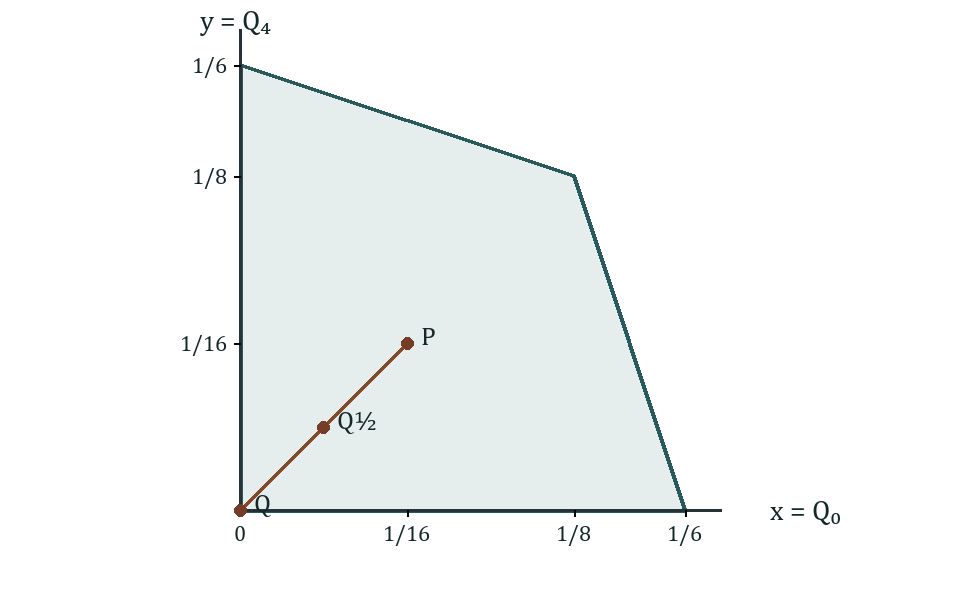
\includegraphics[width=0.63\linewidth,height=\textheight,keepaspectratio,alt={Politopo límite de márgenes para bloques de cuatro puntos. El segmento une el perfil de frontera con la ley de referencia; su punto medio es la mezcla en partes iguales.}]{figures/profile_slice.png}
\par\smallskip\small\textbf{Figura 1.} Politopo límite de márgenes para bloques de cuatro puntos. El segmento une el perfil de frontera con la ley de referencia; su punto medio es la mezcla en partes iguales.
\end{minipage}\end{center}

La tasa también controla las fluctuaciones. Para logaritmos naturales, la desigualdad de Pinsker da \(D(Q\|P)\ge\|Q-P\|_1^2/2\). En efecto, agrupemos las coordenadas con \(Q_j>P_j\) en un solo suceso. La desigualdad de la suma logarítmica acota inferiormente la divergencia por la divergencia binaria de ese suceso. Como función de la primera probabilidad \(u\), la divergencia binaria tiene segunda derivada \(1/[u(1-u)]\ge4\) y se anula junto con su primera derivada en la probabilidad de referencia. La diferencia de probabilidades es \(\|Q-P\|_1/2\). Al aplicar la cota para cerrados a \(\|Q-P\|_1\ge\varepsilon\) se obtiene, para \(\varepsilon>0\) fijo y a lo largo de los órdenes admisibles, \[\limsup_{n\to\infty} b_n^{-1}\log\Pr(\|Q_n-P\|_1\ge\varepsilon)
 \le -\varepsilon^2/2 .\]

\subsection{11. Formalización}\label{formalizaciuxf3n}

El desarrollo en Lean 4.35.0 sigue las dos etapas del argumento. En el Teorema 1.1 la declaración \path{KqR75.PhysicalCompletion.eventually_designFibre_bilateral} reúne las dos estimaciones para las cuotas interiores. La cota superior que admite tipos ausentes se encuentra en \path{KqR75.UpperCounting.eventually_card_designFibre_upper_entropy}. La construcción inferior utiliza la formalización del teorema de omniabsorción de Delcourt y Postle {[}3{]}.

Para el Corolario 10.1, \path{KqR75.ProfileLDP.designProfileLDP_probability} expresa las cotas de probabilidad sobre abiertos y cerrados. La comprobación de axiomas de esta declaración devuelve \path{propext}, \path{Classical.choice} y \path{Quot.sound}.

\subsection{Agradecimientos}\label{agradecimientos}

El autor agradece profundamente a su esposa María Paz y a sus hijos Lucas, Juan Cristóbal, Francisca, Raimundo y Benjamín su amor, paciencia y apoyo.

\subsection{Uso de inteligencia artificial y herramientas computacionales}\label{uso-de-inteligencia-artificial-y-herramientas-computacionales}

Claude, de Anthropic, y ChatGPT/Codex, de OpenAI, se utilizaron para explorar y comprobar argumentos y para preparar el manuscrito.

Certo {[}5{]} se utilizó para explorar casos finitos, comprobar identidades y evaluar construcciones candidatas. Estos cálculos orientaron el desarrollo de los argumentos; las comprobaciones finitas no se trataron como pruebas de enunciados universales.

El autor es responsable de los argumentos, las citas, el código y la exposición. Ningún sistema de IA figura como autor.

\subsection{Referencias}\label{referencias}
\raggedright

{[}1{]} P. Keevash. \emph{Counting designs}. J. Eur. Math. Soc. 20(4) (2018), 903--927, \href{https://doi.org/10.4171/JEMS/779}{doi:10.4171/JEMS/779}.

{[}2{]} J. P. Traverso Gianini. \emph{Counting Steiner triple systems and Latin squares with prescribed color statistics}. Paper II of this series, 2026. \url{https://github.com/jtraverso/color-statistics-steiner-latin}.

{[}3{]} M. Delcourt and L. Postle. \emph{Refined absorption: A new proof of the existence conjecture}. \href{https://arxiv.org/abs/2402.17855}{arXiv:2402.17855}.

{[}4{]} N. Linial and Z. Luria. \emph{An upper bound on the number of Steiner triple systems}. Random Structures Algorithms 43(4) (2013), 399--406, \href{https://doi.org/10.1002/rsa.20487}{doi:10.1002/rsa.20487}.

{[}5{]} J. P. Traverso Gianini. \emph{Certo}. Software, \url{https://github.com/jtraverso/certo-math}.

{[}6{]} J. P. Traverso Gianini. \emph{Entropy and large deviations for Latin squares}. Paper I of this series, 2026. \url{https://github.com/jtraverso/latinon-entropy-ldp/releases/tag/latinon-v1.0}.

{[}7{]} P. Keevash. \emph{Coloured and directed designs}. Building Bridges II, Bolyai Soc. Math. Stud. 28, Springer, 2019, 279--315, \href{https://doi.org/10.1007/978-3-662-59204-5_9}{doi:10.1007/978-3-662-59204-5\_9}. \href{https://arxiv.org/abs/1807.05770}{arXiv:1807.05770}.

{[}8{]} P. Keevash. \emph{The existence of designs II}. \href{https://arxiv.org/abs/1802.05900}{arXiv:1802.05900}.

{[}9{]} M. Kwan, A. Sah and M. Sawhney. \emph{Enumerating matroids and linear spaces}. Comptes Rendus. Mathématique \textbf{361} (2023), 565--575. \href{https://doi.org/10.5802/crmath.423}{doi:10.5802/crmath.423}.

{[}10{]} P. Bennett and T. Bohman. \emph{A natural barrier in random greedy hypergraph matching}. \href{https://arxiv.org/abs/1210.3581}{arXiv:1210.3581}.

\end{document}
